\documentclass[10pt, a4paper]{article}

%%%%%%%%%%%%%%
%  Packages  %
%%%%%%%%%%%%%%


\usepackage{page_format}
\usepackage{special}
\usepackage{hyperref}
\usepackage{tikz}
\usepackage[compat=1.1.0]{tikz-feynman}
%----------------------------------------------------------------------
%\usepackage{amssymb} % Mathematical fonts.
%\usepackage{amsfonts} % Mathematical fonts.
\usepackage[nice]{nicefrac} % Nicer fractions
\usepackage{braket} % Dirac Notation.
\usepackage{bbm} % More bold fonts.
%\usepackage{mathrsfs} % Mathematical fonts.
\usepackage{esint} % Integrals
\usepackage{cancel} % Allows to scratch expressions.
\usepackage{mathtools} % Tools for math formating.
\usepackage{slashed} % Allows to slash individual characters.
\usepackage{xargs} % Better handling of optional arguments for commands
%----------------------------------------------------------------------
%\usepackage{lmodern} % Fonts.
\usepackage{feyn} % Feynman Diagrams in mathmode

%%%%%%%%%%%%%%%%%%%%%%%%%%%
% Mathématiques et physique
%%%%%%%%%%%%%%%%%%%%%%%%%%%%
% SI Units -----------------------
% The package 'siunitx' causes unresolved crashes (as of 22/08/31)
\newcommand{\ampere}{\text{A}}
\newcommand{\bell}{\text{B}}
\newcommand{\celsius}{\degree\text{C}}
\newcommand{\coulomb}{\text{C}}
\newcommand{\degree}{\,^{\circ}}
\newcommand{\farad}{\text{F}}
\newcommand{\electro}{\text{e}}
\newcommand{\gram}{\text{g}}
\newcommand{\henry}{\text{H}}
\newcommand{\hertz}{\text{Hz}}
\newcommand{\hour}{\text{h}}
\newcommand{\joule}{\text{J}}
\newcommand{\kelvin}{\text{K}}
\newcommand{\meter}{\text{m}}
\newcommand{\minute}{\text{m}}
\newcommand{\mole}{\text{mol}}
\newcommand{\newton}{\text{N}}
\newcommand{\ohm}{\Omega}
\newcommand{\pascal}{\text{Pa}}
\newcommand{\rad}{\text{rad}}
\newcommand{\second}{\text{s}}
\newcommand{\tesla}{\text{T}}
\newcommand{\torr}{\text{Torr}}
\newcommand{\volt}{\text{V}}
\newcommand{\watt}{\text{W}}
%
\newcommand{\tera}{\text{T}}
\newcommand{\giga}{\text{G}}
\newcommand{\mega}{~\text{M}}
\newcommand{\kilo}{~\text{k}}
\newcommand{\deci}{\text{d}}
\newcommand{\centi}{\text{c}}
\newcommand{\milli}{\text{m}}
\newcommand{\micro}{\mu}
\newcommand{\nano}{\text{n}}
\newcommand{\pico}{\text{p}}
\newcommand{\femto}{\text{f}}
%
\newcommand{\units}[1]{\text{#1}}
\newcommand{\tothe}[1]{\textsuperscript{#1}}
%
\newcommand{\per}{\text{/}}
%
\newcommand{\Time}[3]{#1\hour~#2\minute~#3\second} % TODO Optional arguments.
\newcommand{\Angle}[3]{#1^{\circ}~#2'~#3''} % TODO Optional arguments.


% Better epsilon -----------------------
\let\oldepsilon\epsilon
\let\epsilon\varepsilon
\let\varepsilon\oldepsilon


% Better \bar -----------------------
\renewcommand{\bar}[1]{\mkern 1.5mu\overline{\mkern-1.5mu#1\mkern-1.5mu}\mkern 1.5mu}


% Équations -----------------------
\newcommand{\al}[1]{\begin{align} #1 \end{align}} % Numbered equation(s),
\newcommand{\eqn}[1]{\begin{align*} #1 \end{align*}} % Number-less equation(s),
\newcommand{\sys}[1]{\begin{dcases*} #1 \end{dcases*}} % System of equations.


% Exponents -----------------------
\newcommand{\Exp}[1]{\text{e}^{#1}}		% e^#
\newcommand{\E}[1]{\times 10^{#1}}		% X 10^#


% Delimiters -----------------------
\newcommand{\p}[1]{\left( #1 \right)}	% (#)
\newcommand{\cro}[1]{\left[ #1 \right]}	% [#]
\newcommand{\abs}[1]{\left| #1\right|}	% |#|
\newcommand{\avg}[1]{\left\langle #1 \right\rangle} % <#>
\newcommand{\acc}[1]{\left\lbrace #1 \right\rbrace} % {#}


% Vectors -----------------------
\newcommand{\ve}[1]{\mathbf{#1}} % Upright bold face.
\newcommand{\vu}[1]{\hat{\ve{#1}}} % Hat vector upright bold face
\newcommand{\tens}{\otimes} % Tensor product
\newcommand{\nablav}{\bm{\nabla}} % Bold gradient


% Trig. functions with automatic formating  -----------------------
\newcommandx{\Sin}[2][1={}]{\text{sin}^{#1}\!\p{#2}}
\newcommandx{\Cos}[2][1={}]{\text{cos}^{#1}\!\p{#2}}
\newcommandx{\Tan}[2][1={}]{\text{tan}^{#1}\!\p{#2}}
\newcommandx{\Csc}[2][1={}]{\text{csc}^{#1}\!\p{#2}}
\newcommandx{\Sec}[2][1={}]{\text{sec}^{#1}\!\p{#2}}
\newcommandx{\Cot}[2][1={}]{\text{cot}^{#1}\!\p{#2}}
\newcommandx{\Arcsin}[2][1={}]{\text{arcsin}^{#1}\!\p{#2}}
\newcommandx{\Arccos}[2][1={}]{\text{arccos}^{#1}\!\p{#2}}
\newcommandx{\Arctan}[2][1={}]{\text{arctan}^{#1}\!\p{#2}}
\newcommandx{\Sinh}[2][1={}]{\text{sinh}^{#1}\!\p{#2}}
\newcommandx{\Cosh}[2][1={}]{\text{cosh}^{#1}\!\p{#2}}
\newcommandx{\Tanh}[2][1={}]{\text{tanh}^{#1}\!\p{#2}}


% Matrices -----------------------
\newcommand{\mat}[1]{\begin{bmatrix} #1 \end{bmatrix}} % Matrices with hooks.
\newcommand{\pmat}[1]{\begin{pmatrix} #1 \end{pmatrix}} % Matrices with parentheses.
\newcommand{\deter}[1]{\abs{\begin{matrix} #1 \end{matrix}}} % Determinant.
\newcommandx{\mO}[2][1={}, 2={}]{ \def\temp{#2}\ifx\temp\empty\ve{O}_{#1}\else\ve{O}_{#1\times #2}\fi}% Zero matrix.
\newcommandx{\mI}[2][1={}, 2={}]{ \def\temp{#2}\ifx\temp\empty\ve{I}_{#1}\else\ve{O}_{#1\times #2}\fi}%  Identity matrix.
\newcommand{\Det}[1]{\text{det}\p{#1}} % det(#)
\newcommand{\Tr}[1]{\text{Tr}\p{#1}} % Tr(#)


% Derivatives -----------------------
\newcommand{\D}{\text{d}} % Differential 'd'.
\newcommandx{\dd}[3][1={},3={}]{\frac{\D^{#3}#1}{\D{#2}^{#3}}} % Total derivative according to #2, #1 is the function and #3 is the order.
\newcommand{\del}{\partial} % Partial 'd'.
\newcommandx{\ddp}[3][1={},3={}]{\frac{\del^{#3}#1}{\del{#2}^{#3}}} % Dérivée partielle selon #2, #1 est la fonction est #3 est l'ordre.
\newcommand{\eval}[1]{\left. {#1} \right|} % Bar on the right of expression.
\newcommand{\delbar}{\slashed{\del}} % Partial Inexact differential.
\newcommand{\dbar}{\dj}% Inexact differential.


% Integrals -----------------------
\newcommand{\intinf}{\int\displaylimits_{-\infty}^{\infty}} % From -00 to 00.
\newcommandx{\Int}[2][1={},2={}]{\int\displaylimits_{#1}^{#2}} % Faster bounded integrals.


% Complex numbers -----------------------
\renewcommand{\Re}[1]{\text{Re}\acc{#1}} % Re{#}
\renewcommand{\Im}[1]{\text{Im}\acc{#1}} % Im{#}


% Sets -----------------------
\newcommand{\N}{\mathbbm{N}} % Natural numbers.
\newcommand{\Z}{\mathbbm{Z}} % Integers.
\newcommand{\Q}{\mathbbm{Q}} % Rational numbers.
\newcommandx{\R}[1][1={}]{\mathbbm{R}^{#1}} % Real numbers.
\newcommandx{\C}[1][1={}]{\mathbbm{C}^{#1}} % Complex numbers.
\newcommandx{\F}[1][1={}]{\mathbbm{F}^{#1}} % Some field.
\newcommand{\M}[3]{\mathbb{M}_{#1\times#2}(#3)}	% Matrices.
\newcommand{\Po}[2]{\mathbb{P}_{#1}(#2)} % Polynomials.
\newcommand{\Lin}{\mathbb{L}} % Linear maps.


% Constants and physical symbols -----------------------
\newcommand{\eo}{\epsilon_0} % epsilon 0.
\renewcommand{\L}{\mathcal{L}} % Lagrangian.

\usepackage{slashed}

% References
\usepackage{biblatex}
\addbibresource{ref.bib}
\usetikzlibrary{positioning}


%%%%%%%%%%%%
%  Colors  %
%%%%%%%%%%%%
% ! EDIT HERE !
\colorlet{chaptercolor}{red!70!black} % Foreground color.
\colorlet{chaptercolorback}{red!10!white} % Background color

%%%%%%%%%%%%%%
% Page titre %
%%%%%%%%%%%%%%%
\title{Homework 1} % Title of the assignement.
\author{\PA} % Your name(s).
\teacher{Yin-Chen He and Timothy Hsieh} % Your teacher's name.
\class{Quantum Matter} % The class title.

\university{Perimeter Institute for Theoretical Physics} % University
\faculty{Perimeter Scholars International} % Faculty
%\departement{<Departement>} % Departement
\date{\today} % Date.


%%%%%%%%%%%%%%%%%%%%%%
% Begin the document %
%%%%%%%%%%%%%%%%%%%%%%
\begin{document}

% Make the title page.
\maketitlepage

% Make table of contents
\maketableofcontents

% Assignment starts here ----------------------------

\footnotesize{

\section{Mean Field theory}

\begin{enumerate}
  \item[(a)] We are interested in the 1-dimensional transverse Ising model. This model is built on a 1-dimensional lattice of $L$ sites with periodic boundary conditions. The positions of the sites are given by integers $i$ modulo $L$. The neighbors of the site $i\ \text{mod}\ L$ are obtained by shifting $i$ by $\pm 1$ and we see that this sets $L$ to be a neighbor of $1 = (L+1)\ \text{mod}\ L$ which implements the periodic boundary condition. From now on, we use $0 \leq i < L$ so the states are directly represented by $i$ in modulo $L$. To each site, we associate a spin degree of freedom represented by states in a two-dimensional Hilbert space $\mathcal{H}_i$. On this local Hilbert space, the Pauli operators expressed in a reference basis $\left\{\ket{0}, \ket{1}\right\}$ are denoted $X_i, Z_i, Y_i$. The full system Hilbert space is $\otimes_i \mathcal{H}_i$ and the Hamiltonian of the transverse Ising model acting on this space reads 
  \begin{align*}
    H = - J \sum_{i=0}^{L-1} Z_i Z_{i+1} - g \sum_{i=0}^{L-1} X_i 
  \end{align*} 
  where $J$ is the ferromagnetic coupling strength between neighboring spins and $g$ is the strength of the transverse magnetic field. If we set $J = 0$, the Hamiltonian $H = - g \sum_{i=0}^{L-1} X_i$ feature a decoupling of the sites. To minimize energy, the spins individually align in the $+X$ direction represented by the state $\ket{+} = (\ket{0} + \ket{1})/\sqrt{2}$ to produce the paramagnetic ground state $\ket{\psi_{\text{PM}}} = \ket{+}^{\otimes L}$. If we set $g = 0$ instead, we get the Hamiltonian $H = - J \sum_{i=0}^{L-1} Z_i Z_{i+1}$ where ferromagnetic interaction favors global alignment of neighboring spins in the $+Z$ or $-Z$ direction. The $\mathbb{Z}_2$ symmetry of the Hamiltonian under flip (represented by the action of $P = \prod_i X_i$) of all spin in the reference basis makes the ferromagnetic ground state degenerate (a fully $+Z$-aligned ground state is mapped by $P$ to a different $-Z$-aligned ground state, contrarily to the paramagnetic groundstate which is left unchanged by $P$: this is a feature of $\mathbb{Z}_2$ symmetry breaking of the ferromagnetic ground state). All the ferromagnetic ground states are given by superpositions of $\ket{\psi^1_{\text{FM}}} = \ket{1}^{\otimes n}$ and $\ket{\psi^0_{\text{FM}}} = \ket{0}^{\otimes L}$.\\

  To do a variational analysis of the evolution of the ground state between $g = 0, J \neq 0$ and $g \neq 0, J = 0$, we consider a parametric curve in the Hilbert space of which the endpoints are $\ket{\psi_{PM}}$ and $\ket{\psi_{FM}^0}$. Noticing that the states at the endpoints are product states of identical states, we take the curve to be successive states in a rotation of each individual spin from the $+Z$ to the $+X$ direction. Such an interpolation, can be written as $\ket{\psi(t)} = (\cos(t/2)\ket{0} + \sin(t/2)\ket{1})^{\otimes L}$ where $t=0$ corresponds to $\ket{\psi_{FM}^0}$ and $t = \pi/2$ to $\ket{\psi_{PM}}$. 

  \item[(b)] We now want to find the point on the curve that minimizes the average energy for a given ratio $g/J$. The first step consists in expressing the average energy for $\ket{\psi(t)}$ as follow 
  \begin{align*}
    \langle H \rangle(t) = \bra{\psi(t)} \left(- J \sum_{i=0}^{L-1} Z_i Z_{i+1}\right) \ket{\psi(t)} +\bra{\psi(t)}\left(- g \sum_{i=0}^{L-1} X_i\right) \ket{\psi(t)}
  \end{align*}
  The expectation value of the ferromagnetic term is 
  \begin{align*}
    &(\cos(t/2)\bra{0} + \sin(t/2)\bra{1})^{\otimes L} \left(- J \sum_{i=0}^{L-1} Z_i Z_{i+1}\right) (\cos(t/2)\ket{0} + \sin(t/2)\ket{1})^{\otimes L} \\
    &= (\cos(t/2)\bra{0}_i + \sin(t/2)\bra{1}_i)(\cdots_{i+1}) \left(- J \sum_{i=0}^{L-1} Z_i Z_{i+1}\right) (\cos(t/2)\ket{0}_i + \sin(t/2)\ket{1}_i)(\cdots_{i+1}) \langle{\neq i, \neq i + 1}|{\neq i, \neq i + 1}\rangle\\
    &= -J \sum_{i=0}^{L-1} \left(\cos(t/2)\bra{0}_i + \sin(t/2)\bra{1}_i\right)(\cdots_{i+1})
    \left(\cos(t/2)\ket{0}_i - \sin(t/2)\ket{1}_i\right)\left(\cos(t/2)\ket{0}_{i+1} - \sin(t/2)\ket{1}_{i+1}\right)\\
    &= -J L \left(\cos^2(t/2)- \sin^2(t/2)\right)\left(\cos^2(t/2)- \sin^2(t/2)\right) = -JL \cos^2(t)
  \end{align*}
  which evaluates to $-JL$ at $t = 0$ (as expected for the ferromagnetic states). To evaluate the transverse field term, we express $\ket{\psi(t)}$ in the $\ket{\pm}$ ($\ket{-} = (\ket{0}-\ket{1})/\sqrt{2}$) eigenbasis of $X_i$ as 
  \begin{align*}
  \ket{\psi(t)} = \left(\cos(t/2)\frac{\ket{+}+\ket{-}}{\sqrt{2}}+\sin(t/2)\frac{\ket{+}-\ket{-}}{\sqrt{2}}\right)^{\otimes L} =  \left((\cos(t/2) + \sin(t/2))\frac{\ket{+}}{\sqrt{2}}+(\cos(t/2)-\sin(t/2))\frac{\ket{-}}{\sqrt{2}}\right)^{\otimes L} 
  \end{align*}
  Then the expectation value of the transverse field term can be written as 
  \begin{align*}
    &\sum_{i=0}^{L-1}\left((\cos(t/2) + \sin(t/2))\frac{\bra{+}_i}{\sqrt{2}}+(\cos(t/2)-\sin(t/2))\frac{\bra{-}_i}{\sqrt{2}}\right) \left(- g  X_i\right)\left((\cos(t/2) + \sin(t/2))\frac{\ket{+}_i}{\sqrt{2}}+(\cos(t/2)-\sin(t/2))\frac{\ket{-}_i}{\sqrt{2}}\right)\langle{\neq i}|{\neq i}\rangle \\
    &= -g \sum_{i=0}^{L-1} \left((\cos(t/2) + \sin(t/2))\frac{\bra{+}_i}{\sqrt{2}}+(\cos(t/2)-\sin(t/2))\frac{\bra{-}_i}{\sqrt{2}}\right) \left((\cos(t/2) + \sin(t/2))\frac{\ket{+}_i}{\sqrt{2}}-(\cos(t/2)-\sin(t/2))\frac{\ket{-}_i}{\sqrt{2}}\right)\\
    &= -g \sum_{i=0}^{L-1} \left((\cos(t/2) + \sin(t/2))^2\frac{1}{2} - (\cos(t/2) - \sin(t/2))^2\frac{1}{2}\right) = -2g L\sin(t/2)\cos(t/2) = -gL \sin(t)
  \end{align*}
  which evaluates to $-gL$ at $t = \pi/2$ (as expected for a fully paramagnetic spin chain). The expectation value of the full Hamiltonian is 
  \begin{align*}
    \langle H \rangle(t) =-JL\cos^2(t) - gL \sin(t). 
  \end{align*}
  \newpage
  \item[(c)] The value $t_\star$ of $t$ that extremizes the expectation value of $H$ for the state considered here is such that 
  \begin{align*}
    0 = \left.\frac{\partial \langle H \rangle(t)}{\partial t}\right|_{t = t_\star} = \cos(t_\star) (2JL\sin(t_\star) - gL) \implies  \cos(t_\star) = 0 \quad \text{or} \quad \sin(t_\star) = \frac{g}{2J}. 
  \end{align*}
  Among the extrema satisfying these conditions, the minima have positive second derivative $\langle H \rangle(t)$ at $t=t_\star$ leading to the additional constraint 
  \begin{align*}
    \left.\frac{\partial^2 \langle H \rangle(t)}{\partial t^2}\right|_{t = t_\star} = 2JL\cos(2t_\star) + gL \sin(t_\star) = > 0 
  \end{align*}
  We now analyze this constraint for $t_\star \in [0, \pi/2]$. In that interval, the only value of $t_\star$ satisfying $\cos(t_\star) = 0$ is $t_\star = \pi/2$ which is associate to the second derivative $L(-2J + g)$. This extremum is only a local minimum for $g > 2J$ (the paramagnetic state becomes a minimum of energy for high enough $g$ compared to $J$). Moving to the extremums satisfying $\sin(t_\star) = \frac{g}{2J}$, we notice that no solution exists for $\frac{g}{2J}>1$ which forces the $t_\star = \pi/2$ to be an absolute minimum in this regime. If $\frac{g}{2J}\leq 1$, we find $t_\star = \arcsin(\frac{g}{2J})$: the $t$ parameter rotates as we increase $g/J$ until it saturates at $\pi/2$ for $\frac{g}{2J}\ge 1$. To check that $\sin(t_\star) = \frac{g}{2J}$ is associated to a minimum (forced to be global if $\frac{g}{2J}\leq 1$), we write 
  \begin{align*}
    2JL\cos(2t_\star) + gL \sin(t_\star) = 2JL (1-2\sin^2(t_\star)) + gL \sin(t_\star) = 2JL \left(1-\frac{g^2}{2J^2}\right) + \frac{g^2}{2J}L = 2JL -\frac{g^2}{J}L + \frac{g^2}{2J}L = \frac{4J^2 - g^2}{2J}L > 0
  \end{align*} 
  implying $4J^2 - g^2 > 0$ which corresponds to $\frac{g}{2J} < 1$ and we indeed have a minimum for the values of $g/J$ complementing the values associated to the $t_\star=\pi/2$ minimum. The curve in the full Hilbert space of the system is given by 
  \begin{align*}
    \ket{\psi(t)} = 
    \begin{cases}
      (\cos\left(\arcsin\left(\frac{g}{2J}\right)/2\right)\ket{0} + \sin\left(\arcsin\left(\frac{g}{2J}\right)/2\right)\ket{1})^{\otimes L},\\
      (\frac{1}{\sqrt{2}}\ket{0} + \frac{1}{\sqrt{2}}\ket{1})^{\otimes L}
    \end{cases}
  \end{align*}
  This state suggests that we have a phase transition at $\frac{g}{2J}$. To analyze the transition further, we calculate the expectation value of $Z_i$ for the energy-minimizing state. We note that this expectation value is the same for all $i$ making the magnetization in the $Z$ direction uniform in the system. This feature is the quantum analog of the statistical mean field theory solution of the Ising model where the free energy is minimized (free energy and energy coincide at zero temperature). We have 
  \begin{align*}
    \bra{\psi(t)}Z_i\ket{\psi(t)} =  \begin{cases}
      (\cos\left(t_\star/2\right)\bra{0} + \sin\left(t_\star/2\right)\bra{1})(\cos\left(t_\star/2\right)\ket{0} - \sin\left(t_\star/2\right)\ket{1}) = \cos\left(t_\star/2\right)^2 - \sin^2\left(t_\star/2\right) = \cos(t_\star) = \sqrt{1- \frac{g^2}{4J^2}},\\
      \left(\frac{1}{\sqrt{2}}\bra{0} + \frac{1}{\sqrt{2}}\bra{1}\right)\left(\frac{1}{\sqrt{2}}\ket{0} - \frac{1}{\sqrt{2}}\ket{1}\right) = 0 
    \end{cases}
  \end{align*}
  As a function of $g/J$, $\bra{\psi(t)}Z_i\ket{\psi(t)}$ (see Fig. \ref{Transition}) reaches $0$ at $\frac{g}{2J} =1$. At this point the derivative of the square root part becomes infinite and we recover the usual divergence of the magnetic susceptibility at a phase transition. 
  \begin{figure}
    \centering
    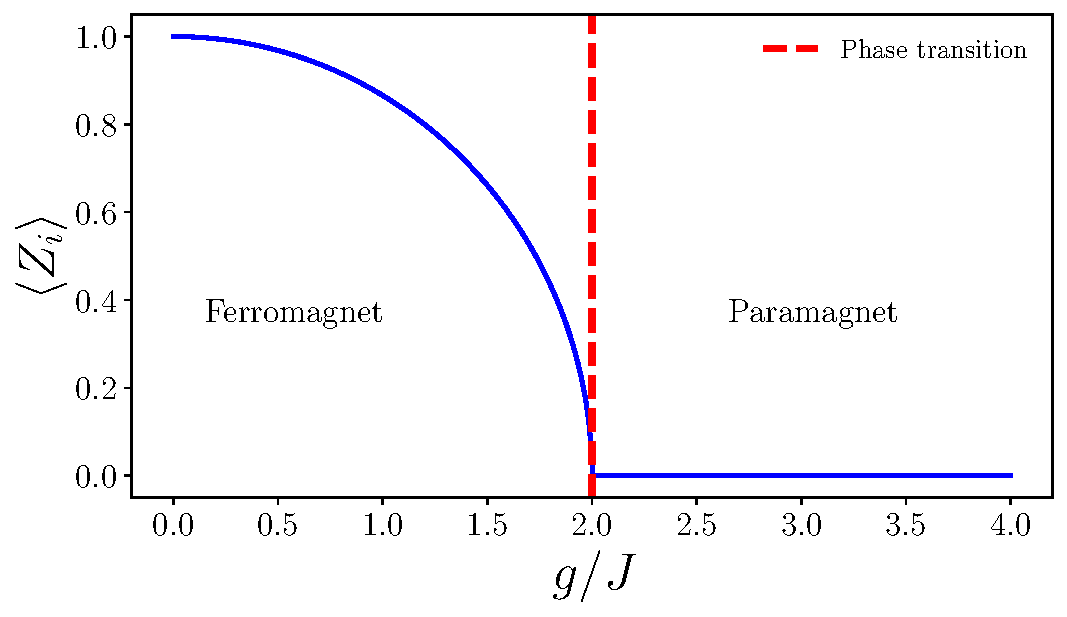
\includegraphics[scale=0.7
    ]{C:/Users/pgraham1/Documents/GitHub/PSI/Quantum_Matter/Homework1/Z_average.pdf}
    \caption{Plot of the expectation value for the local operator $Z_i$ for the product state variational ansatz. This expectation value indicates a phase transition at $g/J =2$ which is different from the $g/J=1$ exact result: this is a feature of the limitations of mean-field theory. To get the expectation value of the operator $\sum_i Z_i$, we can use the central limit theorem because the sites are uncorrelated and share the same probability distribution for their spin states (a feature of the mean-field theory approach taken here).\label{Transition}}
  \end{figure}
\end{enumerate}

\newpage

\section{Matrix Product States}

\begin{enumerate}
  \item[(a)] To go beyond the product state curve from question $1$ which fails to capture entanglement of the ground state, we introduce a tensor network ansatz. This ansatz is called a matrix product state (MPS). To construct it, we define a matrix $M(s)$ for each value of the spin $s\in \{0, 1\}$ in a local basis. The matrices all have size $D \times D$ where $D$ is an integer called bond dimension. The ansats $\ket{\psi}$ projected on a configuration $\ket{s_0 \cdots s_{L-1}}$ yields the wavefuntion $\psi(s_0 \cdots s_{L-1}) = \text{Tr}(M(s_0)\cdots M(s_{L-1}))$ which is symmetric under a shift $s_i \mapsto s_{i+1}$ by cyclic property of the trace. Figure \ref{MPS} shows a schematic representation of a MPS. 
  \begin{figure}
    \centering
    \begin{tikzpicture}
      
      % Tensors
      % Square
      \draw (0,0) rectangle (30pt,30pt);
      %
      \node at (30pt/2,30pt/2) {$M(s_i)$};
    %
      %% Lines
      \draw (30pt, 30pt/2) -- (50pt, 30pt/2);
      \draw (0, 30pt/2) -- (-20pt, 30pt/2);
    %
      \node at (-20pt, 30pt/2) [left] {$D$};
      \node at (50pt, 30pt/2) [right] {$D$};



        \draw (120pt,0pt) rectangle (30pt+120pt,30pt);
        % Label
        \node at (30pt/2+120pt,30pt/2) {$M(s_0)$};
      
        % Lines
        \draw (30pt + 120pt, 30pt/2) -- (50pt + 120pt, 30pt/2);
        \draw (120pt, 30pt/2) -- (-20pt + 120pt, 30pt/2);

        %%%%%%%%%%%%%%%%%%%%%%%%%%

        \draw (210pt,0pt) rectangle (40pt+210pt,30pt);
        % Label
        \node at (40pt/2+210pt,30pt/2) {$M(s_{L-1})$};
      
        % Lines
        \draw (40pt + 210pt, 30pt/2) -- (60pt + 210pt, 30pt/2);
        \draw (210pt, 30pt/2) -- (-20pt + 210pt, 30pt/2);
        \node at (-20pt + 210pt, 30pt/2) [left] {$\cdots$};

        %%%%%%%%%%%%%%%%%%%%%%%%%%%

        
       
        \draw (-20pt + 120pt, 30pt/2) to [bend right=90] (60pt + 210pt, 30pt/2);
    \end{tikzpicture}
    \caption{Schematic representation of a MPS. The diagram on the left represents a single matrix in the multiplication chain taking a $D$-dimensionnal input vector and mapping it to a $D$ dimensional vector output which can then be acted on by the next member of the chain. The diagram on the right represents the MPS: every matrix operation feeds its output to the next and the chain is tied with the trace operation giving it the connectivity of a circle. More precisely, the trace sums over the expectation value of the matrix product for a complete basis of the state in the $D$-dimensionnal vector space on which the matrix acts. For a given expectation value, we can see the matrix chain as propagating the ket on the circle to the bra dual to the initial ket completing the expectation value. \label{MPS}}
  \end{figure}
  
  \item[(b)] A GHZ state $\ket{GHZ} = (\ket{00\cdots 0} + \ket{11\cdots 1})/\sqrt{2}$ can be represented with a MPS. To reach such a representation, we first notice that the wavefunction of the state is $\psi(s_0, \cdots, s_{L-1}) = \frac{1}{\sqrt{2}} \prod_{i=0}^{L-1} \delta_{s_i, 0} + \frac{1}{\sqrt{2}} \prod_{i=0}^{L-1} \delta_{s_i, 1}$. To construct our MPS, we want a matrix $M(0)$ and $M(1)$ such that if any two matrices in the chain are different the trace vanishes. This property is achieved for $D=2$ by matrices of the form 
  \begin{align*}
    M(0) = \begin{pmatrix}
      a & 0 \\
      0 & 0
    \end{pmatrix}, \quad
    M(1) = \begin{pmatrix}
      0 & 0 \\
      0 & b
    \end{pmatrix}
  \end{align*}
  with $a, b\in\mathbb{C}$. Indeed, all the matrices commute and if any of them is different we can bring them together and get $M(1)M(0) = 0$. This zero matrix brings any further matrix multiplication to zero and the trace is forced to vanish. In the two cases where all the matrices are the same, we get a trace of $a^{L}$ for $M(0)$ and $b^{L}$ for $M(1)$. This result indicates that we have to fix $a = b = 2^{-1/(2L)}$ to obtain a normalized GHZ state.  
  \item[(c)] The fully peramagnetic ground state associated to $J = 0$ is given by the product state $\ket{\psi} = (\ket{+})^{\otimes L}$. To express its wave function we write 
  \begin{align*}
    \ket{\psi} = (\ket{+})^{\otimes L} = \bigotimes_{i=0}^{L-1} \frac{1}{\sqrt{2}}(\ket{0}+\ket{1}) = 2^{-L/2} \sum_{\{s_0, \cdots, s_{L-1}\} \in b_L} \ket{s_0, \cdots, s_{L-1}}
  \end{align*}
  where $b_L$ denotes the set of all binary strings of length $L$ (which are all generated by one and only one combination of $\ket{0}, \ket{1}$ obtained in distributing the tensor products). This expansion implies that $\psi(s_0, \cdots, s_{L-1}) = \bra{s_0, \cdots, s_{L-1}}\left.{\psi}\right> = 2^{-L/2}$: the value produced by the MPS should be the same regardless of the combinations. A choice of matrices satisfying this has to remove any dependence of the MPS on the type of spin involved in the chain. We achieve this independence by setting both of the matrices equal to 
  \begin{align*}
    M(0) = M(1) = \begin{pmatrix}
      a&0\\
      0&0
    \end{pmatrix}
  \end{align*}
  with $a \in \mathbb{C}$. The constant $a$ is taken to be $2^{-1/2}$ so that $L$ multiplication of the matrices produces a matrix with only one non-zero diagonal entry $2^{-L/2}$ (equal to the trace).
  \newpage
  \item[(d)] Using first-order perturbation theory, we can expand the ground state up to first order in $J/g$. This expansion will be close to the true ground state for small $J/g$ (we treat the ferromagnetic interaction as a perturbation of the transverse field Hamiltonian which has non-degenerate ground state $\ket{+}^{\otimes L}$). It reads $\ket{\psi} = \ket{+}^{\otimes L} + \frac{J}{4g} \sum_{i=0}^{L-1} \ket{i, (i + 1) \ \text{mod}\ L}$ where $\ket{i, j} = Z_i Z_j \ket{+}^{\otimes L}$ which consists in a state with $+$ flipped to $-$ in locations $i$ and $j$. We aim to construct an MPS representing this approximate groundstate up to $O(J/g)$ (it can be anything beyond that order). Since we are working with an expansion around the paramagnetic ground state, we use the local basis $\{\ket{-}, \ket{+}\}$ and respectively associated to spin labels $s = 0$ and $s = 1$ in our MPS. The wave function of $\ket{\psi}$ is 
  \begin{align*}
    \psi(s_0, \cdots, s_{L-1}) = \prod_{i=0}^{L-1} \delta_{s_i, 1} + \frac{J}{4g} \sum_{j = 0}^{L-1} \delta_{s_{j}, 0}\delta_{s_{(j+1)\ \text{mod}\ L}, 0} \prod_{i=0, i\neq j, (j+1)\ \text{mod}\ L}^{L-1} \delta_{s_i, 1}
  \end{align*}
  The non-zero components of this state are either associated with spin $1$ or with all spin $1$ except exactly two spin $0$. The associated MPS state is required to agree with these properties at $O(J/g)$ but is unconstrained beyond $O(J/g)$. We take matrix $M(1)$ to be 
  \begin{align*}
    M(1) = 
    \begin{pmatrix}
      1&0\\
      0&0
    \end{pmatrix}
  \end{align*}
  so that the component associated with spin $1$ is reached by a chain consisting of $L$ copies of the matrix as desired. Next, we see that the doubly flipped states contribute at $O(J/g)$ and we set $M(0) \propto \sqrt{J/g}$. Then we want to ensure the vanishing of chains with isolated $M(0)$ matrices. Any isolated $M(0)$ will be surrounded by two $M(1)$ matrices and we have  
  \begin{align*}
    M(1) M(0) M(1) = 
    \begin{pmatrix}
      1&0\\
      0&0
    \end{pmatrix}
    \begin{pmatrix}
      a&b\\
      c&d
    \end{pmatrix}
    \begin{pmatrix}
      1&0\\
      0&0
    \end{pmatrix}
    =
    \begin{pmatrix}
      1&0\\
      0&0
    \end{pmatrix}
    \begin{pmatrix}
      a&0\\
      c&0
    \end{pmatrix}
    =
    \begin{pmatrix}
      a&0\\
      0&0
    \end{pmatrix}
  \end{align*}
  where we wrote a fully general form for $M(0)$ in terms of constants $a, b, c, d\in\mathbb{C}$. Setting $a = 0$ makes any isolated $M(0)$ lead to the vanishing of the chain of multiplications as desired. Now we want $M(0)^2$ to resist being mapped to the null matrix when surrounded by $M(1)$. We calculate 
  \begin{align*}
    M(1) M(0)^2 M(1) = 
    \begin{pmatrix}
      1&0\\
      0&0
    \end{pmatrix}
    \begin{pmatrix}
      0&b\\
      c&d
    \end{pmatrix}
    \begin{pmatrix}
      0&b\\
      c&d
    \end{pmatrix}
    \begin{pmatrix}
      1&0\\
      0&0
    \end{pmatrix}= 
    \begin{pmatrix}
      1&0\\
      0&0
    \end{pmatrix}
    \begin{pmatrix}
      bc&\cdots\\
      \cdots&\cdots
    \end{pmatrix}
    \begin{pmatrix}
      1&0\\
      0&0
    \end{pmatrix}
    =
    \begin{pmatrix}
      bc&0\\
      0&0
    \end{pmatrix}
  \end{align*}
  which shows that two neighbouring $M(0)$ resist vanishing. More precisely, since $M(1)$ only has one non-vanishing diagonal element in the same position as the non-vanishing diagonal element of  $M(1)M(0)^2M(1)$, the final contribution of $n$ pairs of $M(0)$ to the trace is $(bc)^n$. Setting $b = c = \sqrt{J/g}$, we get that the trace contribution at order $O(J/g)$ is produced by having $n=0$ or $n=1$. For simplicity, we set $d=0$ and write the final matrix  
  \begin{align*}
    M(0) = \begin{pmatrix}
      0&\sqrt{J/g}\\
      \sqrt{J/g}&0
    \end{pmatrix}.
  \end{align*}
  
  \item[(e)] Here we want to analyze the scaling of the entanglement between components of a bipartition of any MPS state. To perform this analysis we note that the wavefunction of a bipartitionned state can be expressed s $\psi(S, S')$ where $S$ and $S'$ label possible ordered spin sequences in each component of the partition. This wavefunction corresponds component corresponds to the basis state $\ket{S}\otimes\ket{S'}$. Performing a Schmidt decomposition we transform the state to a basis where its entanglement entropy is more transparent before writing it as an MPS state. In general, we can decompose the state of the spin chain as $\ket{\psi} = \sum_{i} \alpha_i \ket{u_i}\ket{v_i}$ where $\ket{u_i}$ ($\ket{v_i}$) is a linear combination of $\ket{S}$ ($\ket{S'}$) states provided by a SVD. The entanglement entropy can be computed from $\alpha_i$. Through a local unitary mapping (this unitary might affect entanglement within each component of the bipartition, but does not entangle/disentangle the components), we can send $\ket{u_i}$, $\ket{v_i}$ to states in our original basis $\ket{S_i}$, $\ket{S_i'}$. The state we obtain is $\ket{\psi} = \sum_{i} \alpha_i \ket{S_i}\ket{S_i'}$. To produce such a state containing non-vanishing components only for the right pairing of $S$ and $S'$, we use the inner produce provided by the trace operation. For two matrices $A$, $B$ element of the vector space $\mathbb{C}^{D\times D}$, we have the inner product $\langle A, B \rangle = \text{Tr}(A^\dagger B)$. We take $A^\dagger(S) = \prod_{q \in S} M(q)$ and $B(S') = \prod_{q \in S'} M(q)$. To produce a Schmidt decomposition using an MPS, we have to find enough sequences $S$ and $S'$ such that $\langle A, B \rangle = \delta(S, S' \text{ paired to S})$. The maximal number of mutually orthogonal states in a $D^2$ dimensional vector space is $D^2$ meaning that no matter the dimension of the Hilbert space described by the MPS, the Schmidt decomposition can have at most $D^2$ terms. Since entanglement is given by $H = -\sum_i |\alpha_i|^2 \log |\alpha_i|^2$, the maximal entanglement for $N$ terms is $H = \sum_i (1/N \log (1/N))$ wich is $2\log(D)$ in our case. Since the entanglement is bounded by a constant that is independent of the size of the system (just like the area of the zero-dimensional boundary of the partition), we have an area law scaling.  
\end{enumerate}
\newpage
\section{The Practical Relevance of Domain Walls}
Consider a sequence of people labeled by numbers $i$ ranging from $0$ to $n$. Person, $j$ is wearing a hat with color $c_j \in \{\text{blue}: 0,\ \text{red} : +1\}$ ($\pm 1$ are numbers associated with each hat color) and sees the colors of the hats of the people with position $i > j$. A game is played by the group: each player must guess the color of their hat and they look for a collective strategy to maximize the number of right answers. The first person has no information on the color of their hat so they use their guess to give information to the rest of the group. They compute $(\sum_{i > 1} c_i)\ \text{mod}\ 2$. If the result is $0$, they "guess" blue and if the result is $1$, they "guess" red. Then the next player knows the parity of the total number of red hats in front of the previous player. They perform the count again which corresponds to the quantity $(\sum_{i > 2} c_i)\ \text{mod}\ 2$. If they find that the parity has not changed the only hat removed from the sum must be a parity-neutral hat: the blue hat. If they find that the parity has changed, their hat must be "parity charged". The third player can update their available relevant information to be exactly the same as the information available to the second player. From the "guess" (always right) of the second player and the initial input of the first player they can compute the parity of the number of red hats including theirs. Then, using the number of red hats visible to them, they repeat the strategy of the first player and win every time. This strategy applies to every player and the only player at risk of "guessing" the wrong color is the first one. 

\section{Acknowledgement}
Thanks to Nikhil for confirming that mean field theory is the source of error on the location of the quantum phase transition in question 1 

Thanks to Mohamed for suggesting to find a \textit{bound} using a Schmidt decomposition in question 2 (e)

Thanks to Nikhil for the discussion about question 2 (e)

Thanks to Nikhil for a hint regarding question 3

}

% References
\makereferences
%-------------------------------------------------------


%%%%%%%%%%%%%%%%%%%%%%%%
% Terminer le document %
%%%%%%%%%%%%%%%%%%%%%%%%
\end{document}
